\capitulo{5}{Aspectos relevantes del desarrollo del proyecto}

En esta sección se van a detallar los aspectos más relevantes que han tenido lugar a lo largo del desarrollo del proyecto. Al tratarse de un desarrolo \textit{software}, y a lo largo de este se han encontrado diferentes retos e inconvenientes, dónde hay que sumarle su posterior ejecución en un \textit{hardware} que posee una pequeña capacidad de conputo. A su vez, se han aplicado buenas prácticas con el objetivo de obtener un resultado de calidad.

\section{Investigación}
El eje principal que posee el proyecto es la \textit{Detección de Objetos}, el cuál a pesar de ser conocido, nunca se había trabajado con él, se puede decir que su conociemnto era puramente teórico. En la misma línea, se desconcoia prácticamente el funcionamiento de la \textit{Raspberry Pi}, la cuál a trabajar de forma internaa con \textit{Raspbian} ha supuesto
una gran ayuda y beneficio al ser un sistema operativo basado en \textit{Debian} el cuál es un sistema que se conocóa de forma previa.
Por todo esto, ha supuesto un doble esfuerzo, especialmente por el primero de ellos, ya que se ha requerido una formación previa par poder conocer el correcto funcionamiento a la hora de entrenar un modelo de detección, así como averiguar cuál era la mejor opción de cara al proyecto.
De cara al objetivo de obtener un mator conocimento acerca de la \textit{Detección de Objetos} se leyeron diferentes \textit{artículos científicos} \cite{Pathak2018,Yang2017, Wu2020}, obteniendo de ellos los suficientes conocimientos sobre su funcionamiento, la calidad de la detección y el redimiento.

\section{Metodología \textit{Scrum}}
Tal y como se comento en el punto \ref{scrum}, el proyecto se ha reliazado siguiendo una metodología ágil, lo cuál nos permite trabajar con \textit{sprints}, de tal manera, que el trabajo a relaizar en cada uno de ellos, se encuentre documentado desde el inicio, para así poder con una mayor eficiencia, pudiendo priorizar las tareas en función de las existentes y contando con diferentes versiones según a la vez que se va siguiendo el desarrollo del proyecto.

Los conocimeientos que se poseían de \textit{Scrum} eran más bien teóricos, pero si que se había tenido la oportunidad de trabajar con ella, durante la realización de las prácticas en empresa.

Una de las principales dificultades encontradas, ha sido la estimación del tiempo que va a ser necesario para pdoer llevarlo a cabo, todo ello apartir de un nombre y descripción, lo cuál ha concluido con resultados no muy exactos, ya que se en algunos casos la estiamción se ha realizado por debajo y en otros por arriba. Si a esto se le suma que ciertas tareas han llevado más tiempo del debido a problemas versiones y de compatibilidades entre sistemas, hay que suamrle que al contar con un determiando número de asiganturas
más la realización de manera paralela de las prácticas, ha conllevado que tareas que de normal llevan pcoo tiempo, han llevado más de lo planeado.

\section{Creación del dataset de entrenamiento y entremiento del modelo de detección}
A lo largo del Grado, a pesar de que se han visto diferentes asignaturas relacionadas con la \textbf{Inteligencia Artificial}, no se ha visto nada relacionado con la \textbf{Visión Artificial}, ni con la \textbf{Detección de Objetos}, siendo esto una desventaja a la hora de crear el dataset del modelo y etiquetarlo con las características correspondientes al algoritmo de detección escogido. Lo que ha conllevado una inversión de horas, de cara a la búsqueda de infromación, así como de las diferentes formas para entrenar el modelo, y con ello la más asequible de cara a requisitos técnicos, debido a que llevar a cabo un entrenamiento de estas características, 
requiere de una tarjeta gráfica potente, así como un equipo los suficientemente potente para llevarlo a cabo, ya que el modelo necesita estar un mínimo de horas entrenando para que el resultado sea medianamente decente y ser funcional.
Debido a esto, las labores de entremiento, se han realizado sobre \textbf{Google Colab}, visto en el Apartado \ref{colab}.

\section{Pruebas realizadas}
A la hora de probar la funcionalidad de modelo que se ha entrenado, se han realizado diferentes pruebas de detección tras su conversión a un modelo \textit{.pb}, el cuál se basa en el grafo de inferencia que calcula \textit{Tensorflow}.
Seguidamente, se comprobó mediante ejecuciones que el modelo es funcional, es decir, que detecta las clases, para las cuáles ha entrenado, detectando imagenes y vídeos.
Con resultados como los que se ven a continuación:

\imagen{coco_detection}{Detección a través del modelo COCO}
\imagen{license_plate_detection}{Detección a través del modelo creado para detectar matrículas}
\imagen{american_plate_detection}{Detección a través del modelo creado para detectar matrículas 2}
\imagen{head_detection}{Detección a través del modelo creado para detectar cabezas}

Tras esto, se realizaron scripts para medir el \textit{accuracy} y para preprocesar las posiciones originales, es decir, convertirlas del formato YOLO al formato \textit{x1, x1, y1, y2}, apto para trabajar con él desde Tensorflow y devolverlas en un único fichero que contenga la ruta de la imagen, el parámetro \textit{x1}, el parámetro \textit{y1}, el parámetro \textit{x2}, el parámetro \textit{y2} y por último el id de la clase que se ha detectado en dicha posición.
Además, por cada imagen que detecta la devuelve representando la posición original, la posición representada por el modelo y el \textit{IoU} entre ambas posiciones.

\clearpage

Tal y como se muestra a continuación junto con los resultados de la evaluación
\imagen{iou2}{Representacioón de la posición original\textit{(verde)}, la posición predecida\textit{(azul)} y el valor del IoU\textit{(amarillo)}.}

\clearpage

Resultados de la evaluación de la calidad del código para el modelo detector de matrículas con un IoU de 0,70:
\begin{figure}[!h]
    \centering
    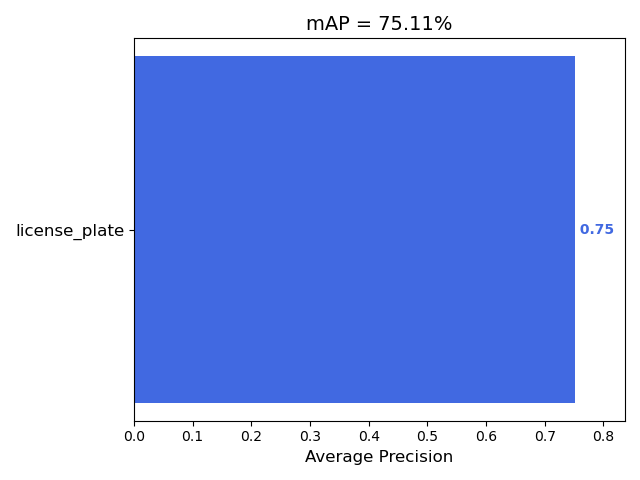
\includegraphics[width=0.4\textwidth]{mAP_lp}
    \caption{mAP del modelo detector de matrículas}\label{fig:mAP_lp}
\end{figure}
\begin{figure}[!h]
    \centering
    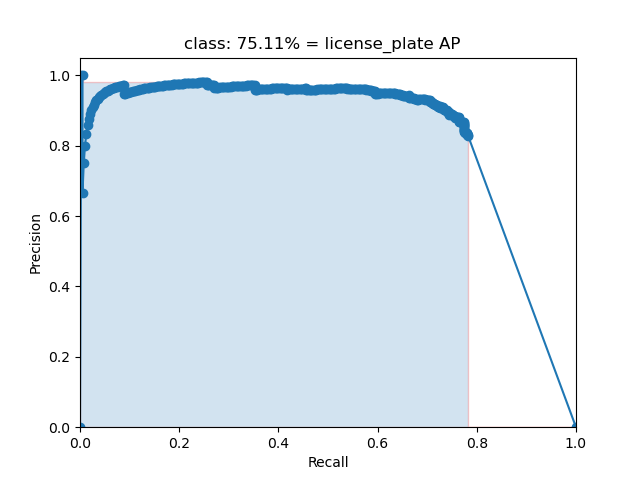
\includegraphics[width=0.4\textwidth]{license_plate_graph}
    \caption{Gráfico \textit{Precission} y \textit{Recall} de la clase \textit{license plate}}\label{fig:license_plate_graph}

\end{figure}
\begin{figure}[!h]
    \centering
    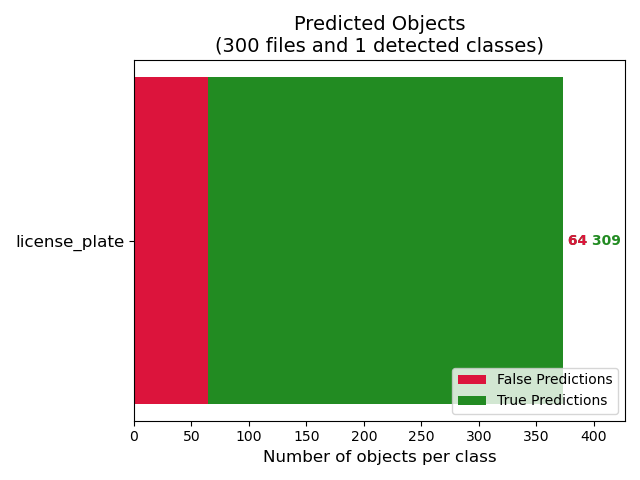
\includegraphics[width=0.4\textwidth]{info_license_plate_predict}
    \caption{Información sobre los \textit{False Predictions} y \textit{True Positives}}\label{fig:info_license_plate_predict}
\end{figure}

\clearpage

Resultados de la evaluación de la calidad del código para el modelo detector de cabezas con un IoU de 0,70:
\begin{figure}[!h]
    \centering
    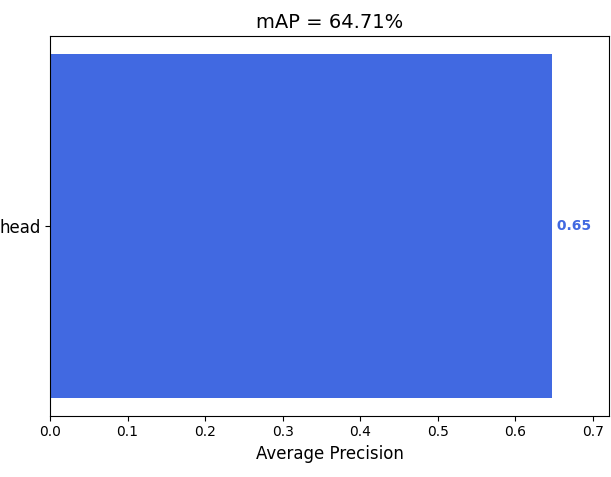
\includegraphics[width=0.4\textwidth]{evalMAP}
    \caption{mAP del modelo detector de cabezas}\label{fig:evalMAP}
\end{figure}

\begin{figure}[!h]
    \centering
    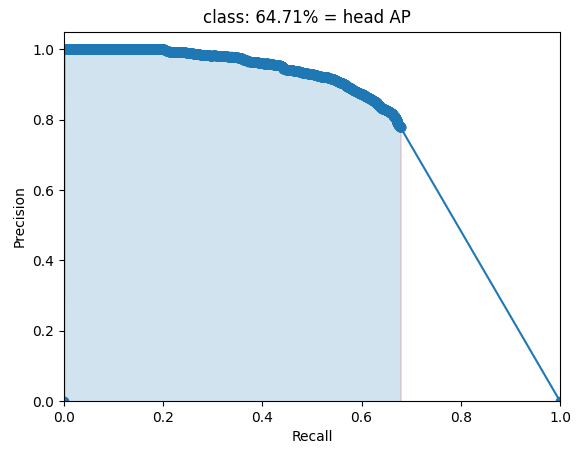
\includegraphics[width=0.4\textwidth]{prEval}
    \caption{Gráfico \textit{Precission} y \textit{Recall} de la clase \textit{head}}\label{fig:prEval}

\end{figure}

\begin{figure}[!h]
    \centering
    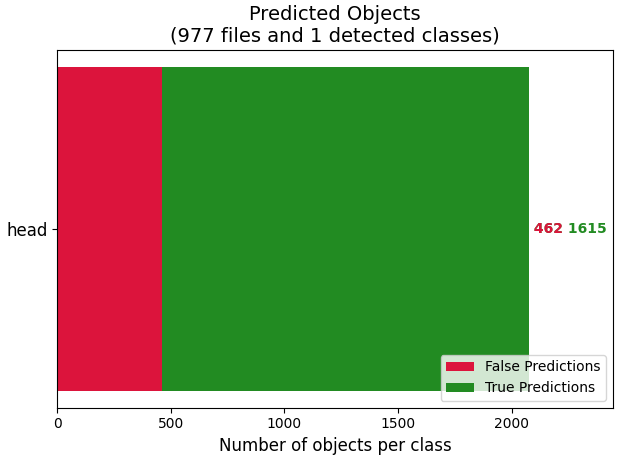
\includegraphics[width=0.4\textwidth]{infoEval}
    \caption{Información sobre los \textit{False Predictions} y \textit{True Positives}}\label{fig:infoEval}
\end{figure}

\clearpage

\section{Resultados evaluación de código} 
Durante el desarrollo se integró una herramienta que permitiesen medir la calidad del código, con el objetivo de controlar la calidad del desarrollo, respecto a los estándares definidos (\textit{ver Apartado }\ref{calidad_codigo}).
En este aprtado veremos los resultados que se han ido obteniendo, los cuáles se ejecutaban automáticamente los análisis al realizarse un \textit{commit}.

\imagen{code_quality_results}{Resultados de la evaluación de la calidad del código}

A través, del dashboard que posee \textit{SonarCloud} para el proyetco, podemos obtener más información sobre la calidad y vulnerabilidades que posee el código.

\imagen{dashboard_sonar}{Resultados mostrados desde el \textit{Dashboard} de SonarCloud} \label{dashboard}

\imagen{evaluacion_sonar}{Gráfico que muestra la evolución del código}

Gracias al uso de esta herramienta, se ha conseguido reducir los \textit{code smells} hasta el punto de poseer una calificación de A.

En la \textit{Figura} \ref{dashboard} se muestra el dashboard de la herramienta, dónde cada uno de los elementos representa:

\begin{list}{\textbullet}{ %
    \addtolength{\itemsep}{-2mm} %
    \setlength{\itemindent}{2mm}}

    \item \textit{Reliability} Representa la fiabilidad del código, en este aparatdo se encuentran los \textit{bugs} que posee el código.
    \item \textit{Maintainability} Representa la mantenibilidad del código, es decir, el código es fácil de mantener y de modificar. En este apartado, se encuentran los \textit{code smells}, los cuáles son indicaciones de que el código, puede suponer un problema en el futuro, ya que a pesar de que posean esta indicación el código no deja de funcionar.
    \item \textit{Security} Indica el nivel de seguridad que posee el código, a este nivel se encuentran las vulnerabilidades del código, las cuáles indican problemas de seguridad tanto a corto como a largo plazo y deben de ser solventados lo antes posible.
    \item \textit{Security Review} Informan sobre las revisiones de seguridad, es decir, informan sobre posibles vulnerabilidades de seguridad, las cuáles deben de ser revisadas por un humano, para calificar si son o no posibles vulnerabilidades de seguridad.
    \item \textit{Coverage} Indica la cobertura del código con respecto a test realizados, es decir, nos muestra el porcentaje de código que supera los tests.
    \item \textit{Duplication Lines} Muestra el porcentaje de lineas que hay duplicadas a lo largo del código.
\end{list}